%% LyX 2.3.4.2 created this file.  For more info, see http://www.lyx.org/.
%% Do not edit unless you really know what you are doing.
\documentclass[11pt]{article}
\usepackage[utf8]{inputenc}
\usepackage[a4paper]{geometry}
\geometry{verbose}
\usepackage{fancyhdr}
\pagestyle{fancy}
\usepackage{float}
\usepackage{amsmath}
\usepackage{graphicx}
\usepackage[unicode=true]
 {hyperref}

\makeatletter

%%%%%%%%%%%%%%%%%%%%%%%%%%%%%% LyX specific LaTeX commands.
%% Because html converters don't know tabularnewline
\providecommand{\tabularnewline}{\\}
\floatstyle{ruled}
\newfloat{algorithm}{tbp}{loa}
\providecommand{\algorithmname}{Algorithm}
\floatname{algorithm}{\protect\algorithmname}

%%%%%%%%%%%%%%%%%%%%%%%%%%%%%% User specified LaTeX commands.
% !TEX TS-program = pdflatex
% !TEX encoding = UTF-8 Unicode

% This is a simple template for a LaTeX document using the "article" class.
% See "book", "report", "letter" for other types of document.

% use larger type; default would be 10pt

% set input encoding (not needed with XeLaTeX)

%%% Examples of Article customizations
% These packages are optional, depending whether you want the features they provide.
% See the LaTeX Companion or other references for full information.

%%% PAGE DIMENSIONS
% to change the page dimensions
 % or letterpaper (US) or a5paper or....
% \geometry{margin=2in} % for example, change the margins to 2 inches all round
% \geometry{landscape} % set up the page for landscape
%   read geometry.pdf for detailed page layout information

% support the \includegraphics command and options

% \usepackage[parfill]{parskip} % Activate to begin paragraphs with an empty line rather than an indent

%%% PACKAGES
% make it possible to include more than one captioned figure/table in a single float
\usepackage{booktabs}% for much better looking tables
\usepackage{array}% for better arrays (eg matrices) in maths
\usepackage{paralist}% very flexible & customisable lists (eg. enumerate/itemize, etc.)
\usepackage{verbatim}% adds environment for commenting out blocks of text & for better verbatim
% make it possible to include more than one captioned figure/table in a single float
% These packages are all incorporated in the memoir class to one degree or another...

%%% HEADERS & FOOTERS
\usepackage{fancyhdr}% This should be set AFTER setting up the page geometry
 % options: empty , plain , fancy
\renewcommand{\headrulewidth}{0pt} % customise the layout...
\lhead{}\chead{}\rhead{}
\lfoot{}\cfoot{\thepage}\rfoot{}

%%% SECTION TITLE APPEARANCE
\usepackage{sectsty}
\allsectionsfont{\sffamily\mdseries\upshape} % (See the fntguide.pdf for font help)
% (This matches ConTeXt defaults)

%%% ToC (table of contents) APPEARANCE
\usepackage[nottoc,notlof,notlot]{tocbibind}% Put the bibliography in the ToC
\usepackage[titles,subfigure]{tocloft}% Alter the style of the Table of Contents
\renewcommand{\cftsecfont}{\rmfamily\mdseries\upshape}
\renewcommand{\cftsecpagefont}{\rmfamily\mdseries\upshape} % No bold!

\usepackage{amsfonts}
%\usepackage{mathcal}

% Pseudocode
\usepackage{algorithm}
\usepackage{algpseudocode}[noend]



%%% END Article customizations

%%% The "real" document content comes below...

\title{Project 1 in FYS3150}
\author{Simon Halstensen, Carl Fredrik Nordbø Knutsen, Jan Harald Aasen \& Didrik Sten Ingebrigtsen}
\date{05.09.2021} % Activate to display a given date or no date (if empty),
         % otherwise the current date is printed 





\makeatother

\begin{document}
\maketitle Project 1 

\href{Github\%20link:\%20https://github.com/sim-hal/FYS3150-Project-1}{Github link: https://github.com/sim-hal/FYS3150-Project-1}

In this project we are solving the following equation: 
\begin{equation}
-\dfrac{d^{2}u}{dx^{2}}=f(x)
\end{equation}
We also know that: 
\begin{itemize}
\item $f(x)=100e^{-10x}$ 
\item $x\in[0,1]$ 
\item $u(0)=u(1)=0$ 
\end{itemize}

\section*{Exercise 1}

I will check that 
\begin{equation}
u(x)=1-(1-e^{-10})x-e^{-10x}
\end{equation}
is a solution to (1) by differentiating $u(x)$ twice.

\[
\dfrac{d^{2}u}{dx^{2}}=\dfrac{d}{dx}(\dfrac{du}{dx})=\dfrac{d}{dx}(-(1-e^{-10})-(-10)e^{-10x})
\]
And since the derivative of a constant is 0, we get that: 
\[
\dfrac{d^{2}u}{dx^{2}}=\dfrac{d}{dx}(10e^{-10x})=-100e^{-10x}
\]
It immediately follows that 
\[
-\dfrac{d^{2}u}{dx^{2}}=100e^{-10x}
\]
This shows that (2) is a solution to equation (1). This solution also
satisfies the boundary conditions specified, as: 
\[
u(0)=1-(1-e^{-10})0-e^{-10\cdot0}=1-1=0
\]
and 
\[
u(1)=1-(1-e^{-10})1-e^{-10\cdot1}=0
\]


\section*{Exercise 2}

The program main.cpp evaluates the exact function $u(x)$ from exercise
1, at points between 0 and 1. It writes the $x$-values and $u(x)$-values
to a .csv-file, named exact\_evaluated.csv. The python script read\_file\_and\_plot.py
reads the values from the .csv-file, and plots the function (see figure
1). 
\begin{figure}[htbp]
\centerline{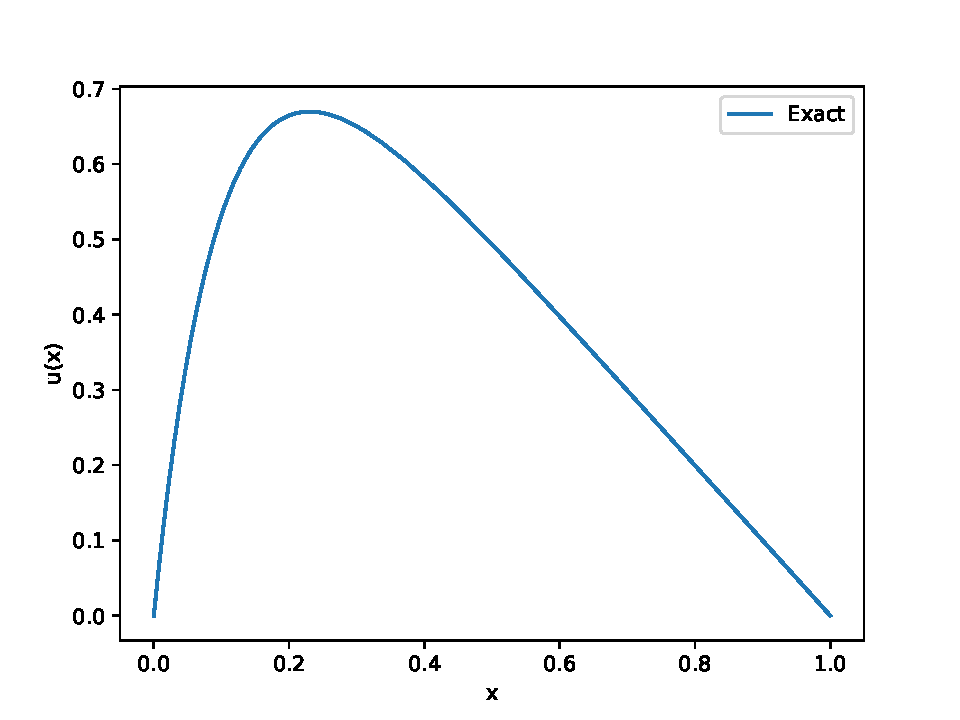
\includegraphics[bb = 0 0 200 100, draft, type=eps]{plots/exact.pdf}}
\caption{Plot of the exact function $u(x)=1-(1-e^{-10})x-e^{-10x}$}
\label{fig} 
\end{figure}


\section*{Exercise 3}

I will derive a discretized version of equation (1) by finding a discretized
approximation of $\dfrac{d^{2}u}{dx^{2}}=u''(x)$. Let $h$ be a step
size, and let $a$ be a point such that $a\in[h,1-h]$. Firstly, evaluate
the 3rd degree Taylor expansion of u(x) about the point $a$ in the
points $a+h$ and $a-h$. 
\[
u(a+h)=u(a)+u'(a)\cdot h+\dfrac{1}{2}u''(a)\cdot h^{2}+\dfrac{1}{6}u'''(a)\cdot h^{3}+\mathcal{O}(h^{4})
\]
\[
u(a-h)=u(a)+u'(a)\cdot(-h)+\dfrac{1}{2}u''(a)\cdot h^{2}+\dfrac{1}{6}u'''(a)\cdot(-h)^{3}+\mathcal{O}(h^{4})
\]
Next, add the two equations, giving the following equality. 
\[
u(a+h)+u(a-h)=2u(a)+u''(a)\cdot h^{2}+\mathcal{O}(h^{4})
\]
The equation can be solved for $u''(a)$ 
\[
u''(a)=\dfrac{u(a+h)-2u(a)+u(a-h)}{h^{2}}+\mathcal{O}(h^{2})
\]
Assuming a sufficiently small value for h, we can approximate and
discretize with $u(ih)\approx v_{i}$. Here, $i\in\{0,1,..,n\}$ (meaning
$n=\dfrac{1}{h}$), and: 
\[
u''(ih)=\dfrac{v_{i+1}-2v_{i}+v_{i-1}}{h^{2}}
\]
Using equation (1), we can rewrite: 
\begin{equation}
h^{2}\cdot f(ih)=-v_{i+1}+2v_{i}-v_{i-1}
\end{equation}
Which is a discretized version of equation (1) with the following
conditions: 
\begin{itemize}
\item $v_{0}=u(0)=0$ 
\item $v_{n}=u(1)=0$. 
\end{itemize}

\section*{Exercise 4}

We will show that you can write the discretized equation as a matrix
equation:

\[
\boldsymbol{A}\vec{v}=\vec{g}
\]
We have eq. (3) from exercise 3, with $i=1,2,\dots,n$. 
\[
\begin{array}{cccccccc}
-v_{0} & 2v_{1} & -v_{2}\\
 & -v_{1} & 2v_{2} & -v_{3}\\
 &  & -v_{2} & 2v_{3} & -v_{4}\\
 &  & \dots & \dots & \dots & \dots & \dots\\
 &  &  &  & -v_{i-3} & 2v_{n-2} & -v_{n-1}\\
 &  &  &  &  & -v_{n-2} & 2v_{n-1} & -v_{n}
\end{array}=h{^{2}}\begin{array}{c}
f_{1}\\
f_{2}\\
f_{3}\\
\vdots\\
f_{n-2}\\
f_{n-1}
\end{array}
\]
we know $v_{0}$and $v_{n}$

\[
\begin{array}{cccccc}
2v_{1} & -v_{2}\\
-v_{1} & 2v_{1} & -v_{3}\\
 & -v_{2} & 2v_{1} & -v_{4}\\
 & \dots & \dots & \dots & \dots & \dots\\
 &  &  & -v_{n-3} & 2v_{n-2} & -v_{n-1}\\
 &  &  &  & -v_{n-2} & 2v_{n-1}
\end{array}=h{^{2}}\begin{array}{c}
f_{1}+v_{0}\\
f_{2}\\
f_{3}\\
\vdots\\
f_{n-2}\\
f_{n-1}+v_{n}
\end{array}\equiv\begin{array}{c}
g_{1}\\
g_{2}\\
g_{3}\\
\vdots\\
g_{n-2}\\
g_{n-1}
\end{array}
\]
We can then seperate out $\vec{v}$ 
\[
\left[\begin{array}{cccccc}
2 & -1\\
-1 & 2 & -1\\
 & -1 & 2 & -1\\
 & \dots & \dots & \dots & \dots & \dots\\
 &  &  & -1 & 2 & -1\\
 &  &  &  & -1 & 2
\end{array}\right]\left[\begin{array}{c}
v_{1}\\
v_{2}\\
v_{3}\\
\vdots\\
v_{n-2}\\
v_{n-1}
\end{array}\right]=\left[\begin{array}{c}
g_{1}\\
g_{2}\\
g_{3}\\
\vdots\\
g_{n-2}\\
g_{n-1}
\end{array}\right]
\]
We now have a known $A$ and $\bar{g}$, so we can solve for $\bar{v}$.

\section*{Exercise 5}

\subsection*{a)}

When the matrix equation in exercise 4 is solved, you get approximate
solutions for all the inner points $x_{i}$ on the interval $(0,1)$.
That is, you get solutions for $v$ for all points except the first
point and the last point. Therefore, if A is a $n\times n$-matrix,
the complete solution $\vec{v}^{*}$ must be of length $m=n+2$, when
you include $v_{0}$ and $v_{n+1}$ (note that we use a different
notation in this problem, with n being the number of intervals and
not the number of points).

\subsection*{b)}

The $n$ equations give solutions $v_{i}$ for all the inner points
$x_{i}$, as explained in exercise a). We do not solve for $v_{n+1}$
or $v_{0}$, as these values are already known (and necessary to compute
values of $v_{i}$ for $i\in\{1,2,...,n\}$ with this method).

\section*{Exercise 6}

\subsection*{a)}

In this exercise, we want to formulate the algorithm for solving $Ax=g$
for a general tridiagonal $A$. This is done in {[}alg \ref{alg:general}{]}.

\begin{algorithm}
\caption{Algorithm for solving $Ax=g$ for a general tridiagonal matrix $A$.
$a$, $b$ and $c$ represent the sub-, main- and superdiagonal. Solving
it means taking in $A$ and $g$, and returning $x$.}
\begin{algorithmic}[0] \Procedure{tridiagonal solver}{a, b,
c, g, N} \State $\tilde{b}_{0}\gets b_{0}$ \State $\tilde{g}_{0}\gets g_{0}$
\For{$i\in(1,N)_{\mathbb{N}}$} \State $\tilde{b}_{i}\gets b_{i}-\frac{a_{i}}{\tilde{b}_{i-1}}c_{i-1}$
\State $\tilde{g}_{i}\gets g_{i}-\frac{a_{i}}{\tilde{b}_{i-1}}\tilde{g}_{i-1}$
\EndFor \State $x_{N}\gets\frac{\tilde{g}_{N}}{\tilde{b}_{N}}$
\For{$i\in(N-1,0)_{\mathbb{N}}$} \State $x_{i}\gets\frac{\tilde{g}_{i}-c_{i}x_{i+1}}{\tilde{b}_{i}}$
\EndFor \State \Return $x$ \EndProcedure \end{algorithmic} \label{alg:general} 
\end{algorithm}


\subsection*{b)}

The number of floating point operations (FLOPs) in the general algorithm
in {[}alg \ref{alg:general}{]} is $2\cdot3N=6N$, where $N$ is the
size of the matrix, for forward substitution. For back substitution,
we have $3N$ FLOPs. In total, the algorithm has $9N=\mathcal{O}(N)$
FLOPs.

\section*{Exercise 7}

\subsection*{b)}

The plot that can be seen in {[}fig:\ref{fig:approx}{]} shows how
higher values of $n$ lead to better approximations.

\begin{figure}
\centerline{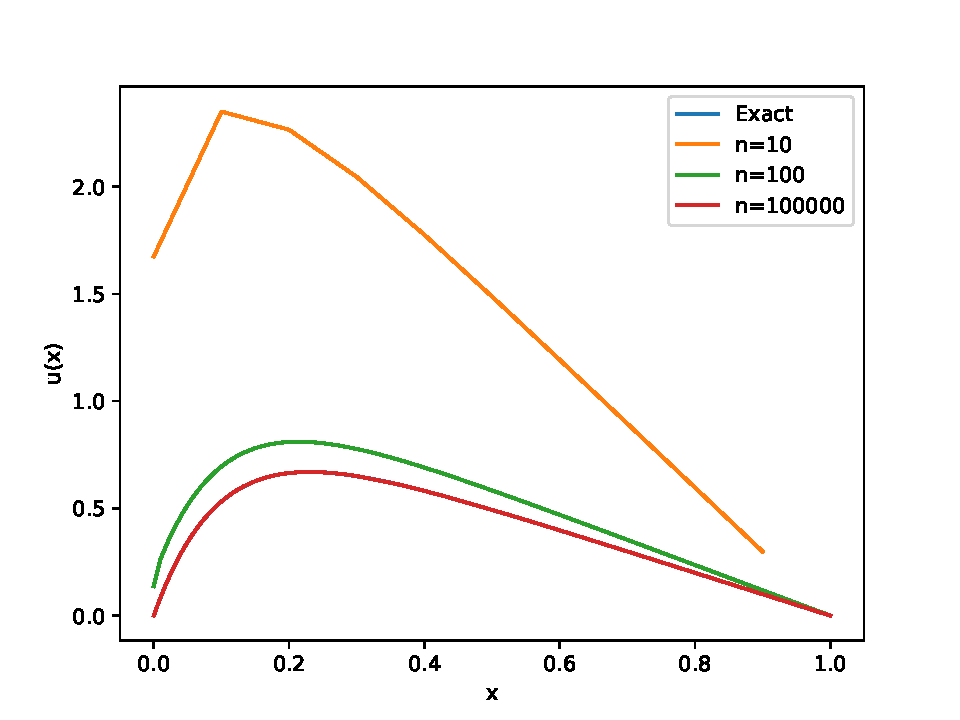
\includegraphics[bb = 0 0 200 100, draft, type=eps]{plots/exact-10-100-100000.pdf}}
\caption{Plot of the exact function $u(x)=1-(1-e^{-10})x-e^{-10x}$ against
numerical approximations with different amount of steps ($n$)}
\label{fig:approx} 
\end{figure}


\section*{Exercise 8}

\subsection*{a) and b)}

The plot of error for different numerical approximations to the equation
can be seen in {[}fig:\ref{fig:error}{]}. 
\begin{figure}
\label{fig:error} 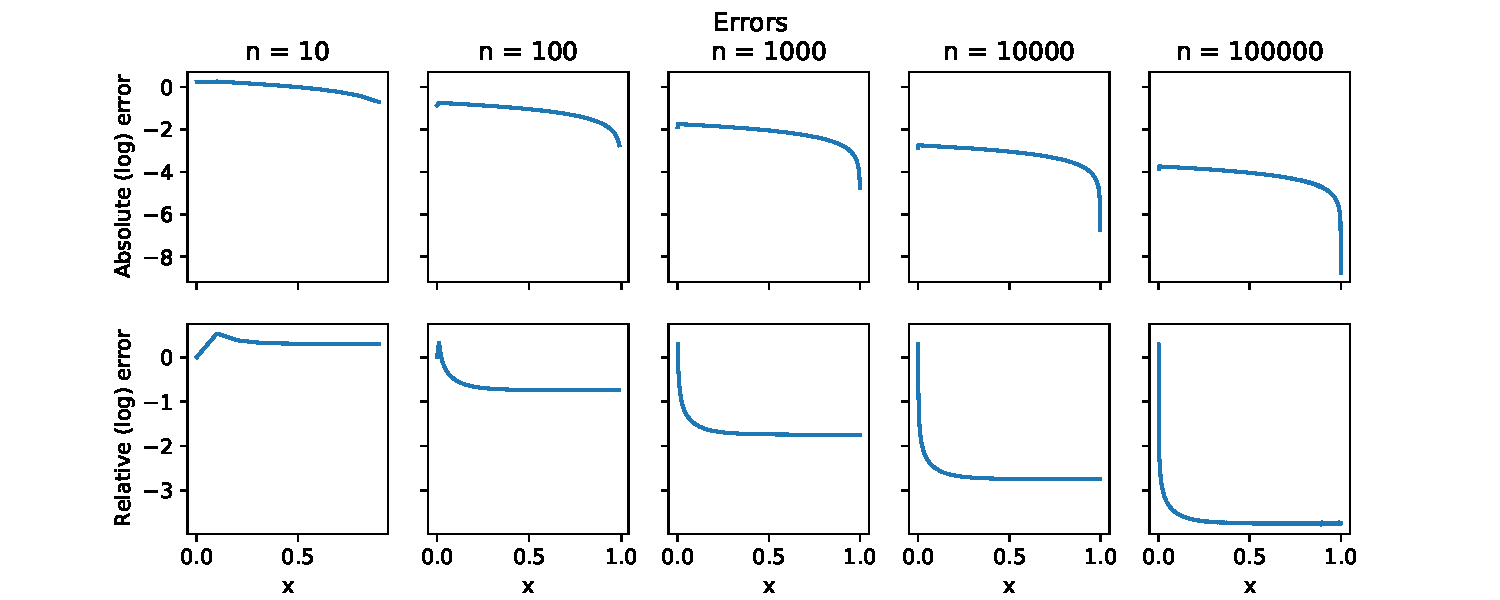
\includegraphics[width=1\textwidth,bb = 0 0 200 100, draft, type=eps]{plots/errors.pdf}
\caption{Plot of absolute and relative log errors for different values of $n$.}
\end{figure}


\subsection*{c)}

The maximum error for numerical approximations with different $n$
values, can be seen in {[}tab:\ref{tab:maxerr}{]}. Here, it is obvious
that higher $n$-values lead to lower errors, and that multiplying
$n$ by $10$ is roughly equivalent to removing $2/3$ of the maximum
absolute error. The maximum relative error however, is reduced by
a lot less, indicating that there is still some significant error
when the actual value is very low.

\begin{table}
\centering{}%
\begin{tabular}{cccccc}
n:  & 10  & 100  & 1000  & 10000  & 100000 \tabularnewline
\hline 
 & 1.296  & 0.4745  & 0.1747  & 0.06427  & 0.02364 \tabularnewline
 & 1.705  & 1.383  & 1.354  & 1.352  & 1.351 \tabularnewline
\end{tabular}\caption{Maximum absolute and relative error in a time step, for each $n$.}
\label{tab:maxerr} 
\end{table}


\section*{Exercise 9}

In this exercise, we want to specialize our algorithm from problem
6, to the case where our $A$ matrix is specified by the signature
$(-1,2,-1)$. This means that the matrix is tridiagonal, and with
$a=(-1,-1,\ldots,-1)$, $b=(2,2,\ldots,2)$ and $c=(-1,-1,\ldots,-1)$.

\subsection*{a)}

Firstly, we want to describe how our specialized algorithm looks.
If we start of with our general algorithm {[}alg \ref{alg:general}{]},
and set $a$, $b$, and $c$ to be our specific vectors, we find that
$\tilde{b}$ is 
\begin{align*}
\tilde{b}_{i} & =b_{i}-\frac{a_{i}}{\tilde{b}_{i-1}}c_{i-1}=2-\frac{(-1)}{\tilde{b}_{i-1}}\cdot(-1)\\
 & =2-\frac{1}{\tilde{b}_{i-1}}=\begin{cases}
\frac{i+3}{i+2} & i>1\\
2 & i=1
\end{cases}
\end{align*}

In the expression for $v$, we also retrieve elements from the $c$
vector, which now always gives the value $-1$. Therefore, it can
be simplified slightly: 
\begin{align*}
v_{i} & =\frac{\tilde{g}_{i}-c_{i}v_{i+1}}{\tilde{b}_{i}}=\frac{\tilde{g}_{i}+v_{i+1}}{\tilde{b}_{i}}
\end{align*}

$\tilde{g}$ can also be rewritten, and $v$ can be worked more on,
so that neither retrieve data from $\tilde{b}$, making the vector
obsolete. This will store and retrieve less data, but require more
FLOPs, so we choose not to.

\subsection*{b)}

This new algorithm, which calculates $\tilde{b}$ in a simpler way,
saves $2N$ FLOPs through simpler calculation of $\tilde{b}$, and
$N$ for $v$, meaning the full algorithm goes from $9N$ to $6N$
FLOPs. This is still $\mathcal{O}(N)$, so the improvement is likely
noticeable, but not very important.

% Likewise, by inserting our new $\tilde{b}$, $\tilde{g}$ becomes

% \begin{align*}
% \tilde{g}_i & = g_i + \frac{\tilde{g}_{i-1}}{\tilde{b}_{i-1}} = \begin{cases} g_i + \frac{i+1}{i+2} \tilde{g}_{i-1} & i > 2 \\ g_i + \frac{\tilde{g}_{i-1}}{2} & i = 2 \\ g_i & i = 1 \end{cases} \\
% \end{align*}

\section*{Exercise 10}

We see that execution time increases linearly as expected, and the
execution time for the special is lower than the generel. 

\begin{tabular}{|c|c|c|}
\hline 
N  & time generel (s) & time special (s)\tabularnewline
\hline 
\hline 
100 & 3.418E-06  & 3.278E-06 \tabularnewline
\hline 
1000 & 2.855E-05  & 1.8821E-05 \tabularnewline
\hline 
10000 & 0.000256742  & 0.000181819 \tabularnewline
\hline 
100000 & 0.00255639  & 0.00192241 \tabularnewline
\hline 
1000000 & 0.0258861  & 0.0238919 \tabularnewline
\hline 
\end{tabular}

Table of execution times 

\section*{Exercise 11}

LU decomposition has the same complexity as matrix multiplication
(). The Lu therefor recuier more FLOPs than the. 

The number of floating point operations (FLOPs) in the general algorithm
in {[}alg \ref{alg:general}{]} is $2\cdot3N=6N$, where $N$ is the
size of the matrix, for forward substitution. For back substitution,
we have $3N$ FLOPs. In total, the algorithm has $9N=\mathcal{O}(N)$
FLOPs. 
\end{document}
